\documentclass[./../main_file.tex]{subfiles}

\begin{document}
	
	Phần này giới thiệu về bộ công cụ kiểm thử tự động hóa Selenium.
	
	\subsection{Selenium là gì?}
	
	Selenium là một trong những bộ công cụ kiểm thử tự động giao diện người dùng (User Interface) có mã nguồn mở được sử dụng rộng rãi nhất. Ban đầu nó được phát triển bởi Jason Huggins vào năm 2004 như một công cụ nội bộ tại Thought Works.
	
	Selenium không thể kiểm thử tự động các ứng dụng trên desktop vì nó chỉ có thể được sử dụng trong các trình duyệt. Selenium được coi là một trong những bộ công cụ được yêu thích nhất để kiểm thử tự động các ứng dụng web vì nó hỗ trợ hầu hết các trình duyệt web phổ biến như Google Chrome 12+, Internet Explorer 7, 8, 9, 10, Safari 5.1+, Opera 11.5, Firefox 3+ và hệ điều hành như Windows, Mac, Linux/Unix. Hơn nữa, nó còn hỗ trợ các hệ điều hành cho ứng dụng di động như iOS và Android.
	
	Selenium cũng cung cấp khả năng tương thích với các ngôn ngữ lập trình khác nhau như Java, C\#, Perl, JavaScript, Ruby, Python, PHP,... phổ biến nhất vẫn là Java và C\#. Người kiểm thử có thể chọn bất cứ ngôn ngữ nào mà Selenium hỗ trợ để thiết kế các ca kiểm thử. Nếu ứng dụng đang được kiểm thử được viết bằng PHP thì người kiểm thử không nhất thiết phải viết mã Selenium bằng PHP, có thể thay bằng Java, Ruby,... Do đó sử dụng Selenium rất thuận lợi bởi tính linh hoạt của nó.
	
	\begin{figure}[H]
		\centering
		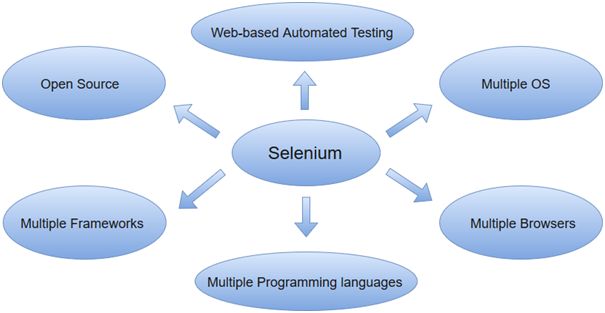
\includegraphics[width=\linewidth]{./images/image1.png}
		\caption{Framework Selenium}
	\end{figure}
	
	Selenium có thể được sử dụng để tự động hóa các ca kiểm thử chức năng và tích hợp với các công cụ kiểm thử tự động như Maven, Jenkins và Docker để đạt được khả năng kiểm thử liên tục. Nó cũng có thể được tích hợp với các công cụ như TestNG và JUnit để quản lý các ca kiểm thử và tạo báo cáo.
	
	\subsection{Các công cụ của Selenium}
	
	Sản phẩm đầu tiên trong bộ kiểm thử Selenium là Selenium Remote Control (hay còn gọi là Selenium 1). Do tồn tại một số hạn chế và sự hợp nhất sau với WebDriver (dẫn đến Selenium 2), nó đã sớm không còn được sử dụng và hỗ trợ nữa. Vào năm 2016, Selenium 3 đã được phát hành, loại bỏ Selenium RC nhưng mở rộng danh sách các trình duyệt được hỗ trợ và khả năng kiểm thử di động. Vào tháng 2 năm 2021, bản phát hành beta đầu tiên của Selenium 4 đã được công bố.
	
	\begin{figure}
		\centering
		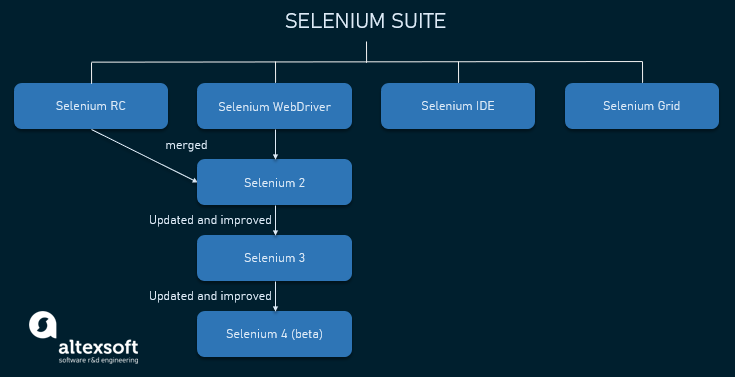
\includegraphics[width=\linewidth]{./images/image7.png}
		\caption{Bộ công cụ Selenium}
	\end{figure}

	Selenium IDE (Môi trường phát triển tích hợp) chủ yếu là một công cụ record and playback. Nó là một Add-on hay Extension có sẵn cho cả Firefox và Chrome, tạo ra ca kiểm thử nhanh chóng thông qua chức năng record and playback. Không cần phải học bất kỳ một ngôn ngữ kịch bản kiểm thử nào nhưng vẫn có thể tạo ra các ca kiểm thử. 
	
	Trong trường hợp làm việc với Selenium Remote Control (Điều khiển từ xa), người kiểm thử phải có kiến thức tốt về ít nhất một ngôn ngữ lập trình. Công cụ này cho phép tạo ra các ca kiểm thử bằng ngôn ngữ kịch bản đã chọn. Server và Client là hai thành phần chính của Selenium RC. Kiến trúc của nó rất phức tạp và tồn tại nhiều hạn chế.
	
	Selenium WebDriver là phiên bản nâng cấp của Selenium RC. Nó ra đời để khắc phục những hạn chế gặp phải trong Selenium RC. Mặc dù nó là một phiên bản nâng cấp từ RC, nhưng kiến trúc của nó hoàn toàn khác với RC. Giống như Selenium RC, Selenium WebDriver cũng hỗ trợ nhiều nền tảng lập trình để mang lại sự linh hoạt và yêu cầu người kiểm thử phải biết ít nhất một ngôn ngữ lập trình nào đó.
	
	Selenium Grid là một công cụ được sử dụng để thực thi đồng thời các ca kiểm thử trên các trình duyệt và hệ điều hành khác nhau cùng một lúc. Công cụ này giúp kiểm tra khả năng tương thích giữa các trình duyệt rất dễ dàng. Đến nay, Selenium Grid đã ra mắt phiên bản 4, tuy nhiên phiên bản này vẫn đang trong quá trình thử nghiệm. Để tránh lỗi phát sinh trong quá trình kiểm thử, nên chọn phiên bản ổn định mới nhất là 3.14.
	
	\subsection{Selenium IDE}
	
	Selenium IDE (Môi trường phát triển tích hợp) là công cụ record and playback mà bất cứ ai cũng có thể sử dụng từ tester đến lập trình viên, thậm chí là những người không có chuyên môn về lập trình bởi đây là một công cụ dễ sử dụng, không yêu cầu bất cứ kiến thức về lập trình, chỉ cần thêm tiện ích mở rộng Selenium IDE từ cửa hàng vào trình duyệt.
	
	Selenium IDE cung cấp một GUI (Giao diện đồ họa người dùng) để dễ dàng ghi lại các tương tác của người dùng với trang web, cho phép người dùng hoặc lập trình viên tạo ra các ca kiểm thử, bộ kiểm thử và chỉnh sửa nó theo yêu cầu của họ.
	
	Môi trường phát triển cũng cung cấp khả năng chuyển đổi các ca kiểm thử sang các ngôn ngữ lập trình khác nhau. Trước đó, Selenium chỉ có sẵn cho người dùng Firefox. Nhưng giờ đây, từ phiên bản nâng cấp 3.12.0 vào ngày 16 tháng 7 năm 2019, cộng đồng Selenium đã giới thiệu Selenium IDE cho Chrome. Sau cùng, người dùng Chrome cũng được cung cấp đầy đủ các tính năng của Selenium IDE như trên Firefox. Ảnh chụp màn hình bên dưới cho biết cách Selenium IDE trên Chrome xuất hiện sau khi nhập tên dự án và URL cơ sở.
	
	\begin{figure}[H]
		\centering
		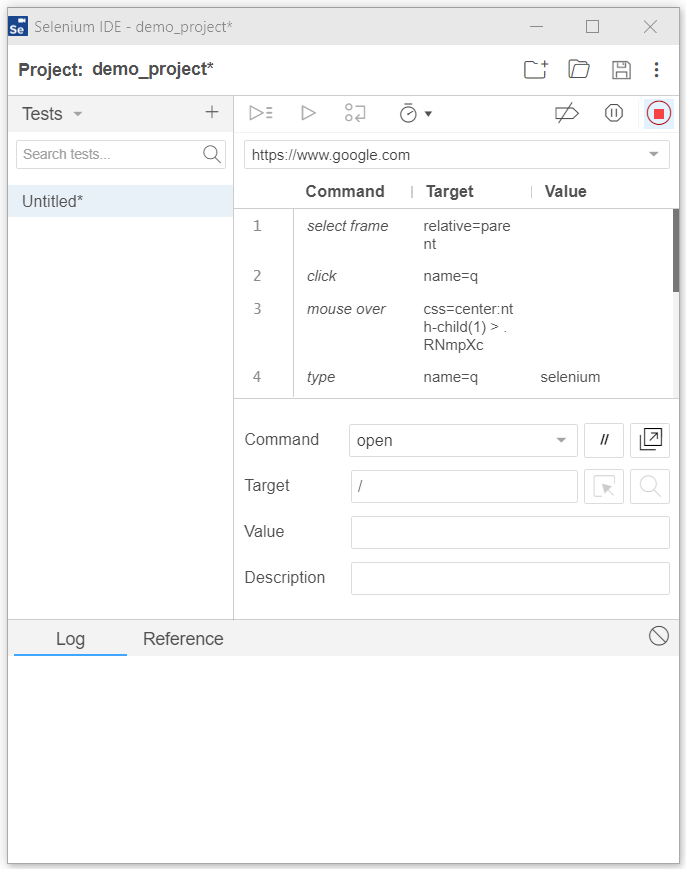
\includegraphics[width=0.7\linewidth]{./images/image10.png}
		\caption{Giao diện Selenium IDE}
	\end{figure}

	Sau khi nhập URL của trang web, quá trình record bắt đầu và tất cả các tương tác với trang web được ghi lại và phân loại thành ba loại chính là:
	
	\begin{itemize}
		\item Command: câu lệnh
		\item Target: vị trí của phần tử
		\item Value: giá trị kiểm thử so với kết quả thực tế
	\end{itemize}

	Tham số target và value có thể có hoặc không và chúng phụ thuộc vào command.
	
	\subsubsection{Tính năng của Selenium IDE}
	
	Các tính năng mà Selenium IDE cung cấp đều nằm trên thanh công cụ giúp người dùng có thể dễ dàng kiểm soát quá trình thực thi các ca kiểm thử:
	
	\begin{itemize}
		\item Speed Control - Kiểm soát tốc độ của các ca kiểm thử
		\item Run All - Thực thi toàn bộ các ca kiểm thử
		\item Run - Thực thi ca kiểm thử hiện tại
		\item Pause/Resume - Tạm dừng và tiếp tục một ca kiểm thử cụ thể
		\item Step - Bước vào từng lệnh cụ thể trong test script
		\item Rollup - Nhóm tất cả các lệnh Selenese lại với nhau và yêu cầu chúng thực thi một thao tác duy nhất
	\end{itemize}

	\subsubsection{Selenese là gì?}
	
	Selenese là ngôn ngữ được sử dụng để viết các lệnh trong Selenium. Các lệnh Selenium này được sử dụng để kiểm tra các ứng dụng web. Dựa trên các thẻ HTML từ giao diện người dùng, người kiểm thử có thể kiểm tra sự tồn tại của chúng. Các lệnh giúp Selenium hiểu những hành động hoặc thao tác cần thực hiện.
	
	\subsubsection{Phân loại các lệnh Selenium}
	
	Các lệnh Selenium được phân loại thành ba loại:
	
	\begin{itemize}
		\item Actions - Gồm các lệnh thao tác trực tiếp với các phần tử : click, type,...
		Ví dụ: Nhấp chuột vào một số liên kết hoặc tùy chọn trên trang.
		
		\item Accessors - Gồm các lệnh để lưu giá trị vào một biến: store, storeTitle,...
		Ví dụ: Lệnh “storeTextPresent” - nếu văn bản được tìm thấy trên trang thì nó sẽ lưu trữ “true”, ngược lại lưu trữ “false”.
		
		\item Assertions - So sánh kết quả mong đợi và thực tế. Chia thành 3 chế độ: Assert, Verify và WaitFor. Chúng hoạt động giống như một bảng checkpoint, nếu cả hai giá trị đều bằng nhau thì ca kiểm thử đó trả về “pass”, ngược lại trả về “false”. Do đó, Assertions giúp xác minh trạng thái của ứng dụng sau khi thực hiện test case có phù hợp với trạng thái mong muốn hay không
		Ví dụ: VerifyText, waitForPageToLoad.
	\end{itemize}

	\subsubsection{Ưu điểm}
	
	\begin{itemize}
		\item Tự động ghi lại các ca kiểm thử dựa trên các tương tác với trình duyệt
		\item Mang lại sự linh hoạt trong việc thực thi các ca kiểm thử. Người kiểm thử có thể chạy toàn bộ các ca kiểm thử hoặc thực thi một ca kiểm thử duy nhất
		\item Hoạt động dựa trên tập hợp các câu lệnh Selenese phong phú, giúp IDE hiểu được những gì cần phải thực hiện
		\item Cho phép người kiểm thử đặt các breakpoint để gỡ lỗi các ca kiểm thử cụ thể
		\item Tái sử dụng các ca kiểm thử bằng lệnh run.
		\item Sử dụng nhiều bộ định vị cho từng phần tử trong IDE đảm bảo thực thi thành công
	\end{itemize}
	
	\subsubsection{Nhược điểm}
	
	\begin{itemize}
		\item Không thích hợp để kiểm thử với dữ liệu lớn
		\item Không thể kiểm tra kết nối với cơ sở dữ liệu
		\item Không thể xử lý phần động của các ứng dụng web
		\item Không hỗ trợ chụp ảnh màn hình khi kiểm thử không thành công
		\item Không có sẵn tính năng để tạo báo cáo kết quả
	\end{itemize}
	
	\subsection{Selenium WebDriver}
	
	Selenium WebDriver là một web framework cho phép thực thi các ca kiểm thử trên nhiều trình duyệt. Công cụ này được sử dụng để kiểm thử tự động các ứng dụng web và  xác minh rằng chúng hoạt động như ta như mong đợi.
	
	Selenium WebDriver cho phép lựa chọn ngôn ngữ lập trình để tạo ra các kịch bản kiểm thử. Đây là phiên bản nâng cấp so với Selenium Remote Control để khắc phục một số hạn chế tồn tại trước đó. Selenium WebDriver không có khả năng xử lý các thành phần cửa sổ, nhưng nhược điểm này có thể được khắc phục bằng cách sử dụng các công cụ như Sikuli, Auto IT,...
	
	Kiến trúc WebDriver được tạo thành từ bốn thành phần chính: Thư viện Selenium Client, giao thức JSON qua HTTP, trình điều khiển trình duyệt và các trình duyệt.

	\begin{description}
		\item[Thư viện Selenium Client] Selenium cung cấp khả năng tương thích cho nhiều ngôn ngữ lập trình như Ruby, Python, Java, C\#,... đều có trên trang web chính thức của Selenium.
		\item[JSON Wire Protocol] Nhà phát triển Selenium WebDriver đã tạo ra 1 cơ chế vận chuyển gọi là JSON Wire Protocol. Đây là một giao thức có thể vận chuyển tất cả các yếu tố cần thiết đến đoạn mã code điều khiển nó. Nó giao tiếp bằng cách sử dụng REST API giữa các máy chủ của HTTP. Mỗi một trình điều khiển trình duyệt sẽ có một máy chủ HTTP riêng biệt.
		\item[Trình điều khiển trình duyệt] Selenium cung cấp các trình điều khiển cụ thể cho từng trình duyệt.
		\item[Các trình duyệt] Selenium WebDriver hỗ trợ cho nhiều trình duyệt như Chrome, Firefox, Safari, Internet Explorer,...
	\end{description}

	\begin{figure}
		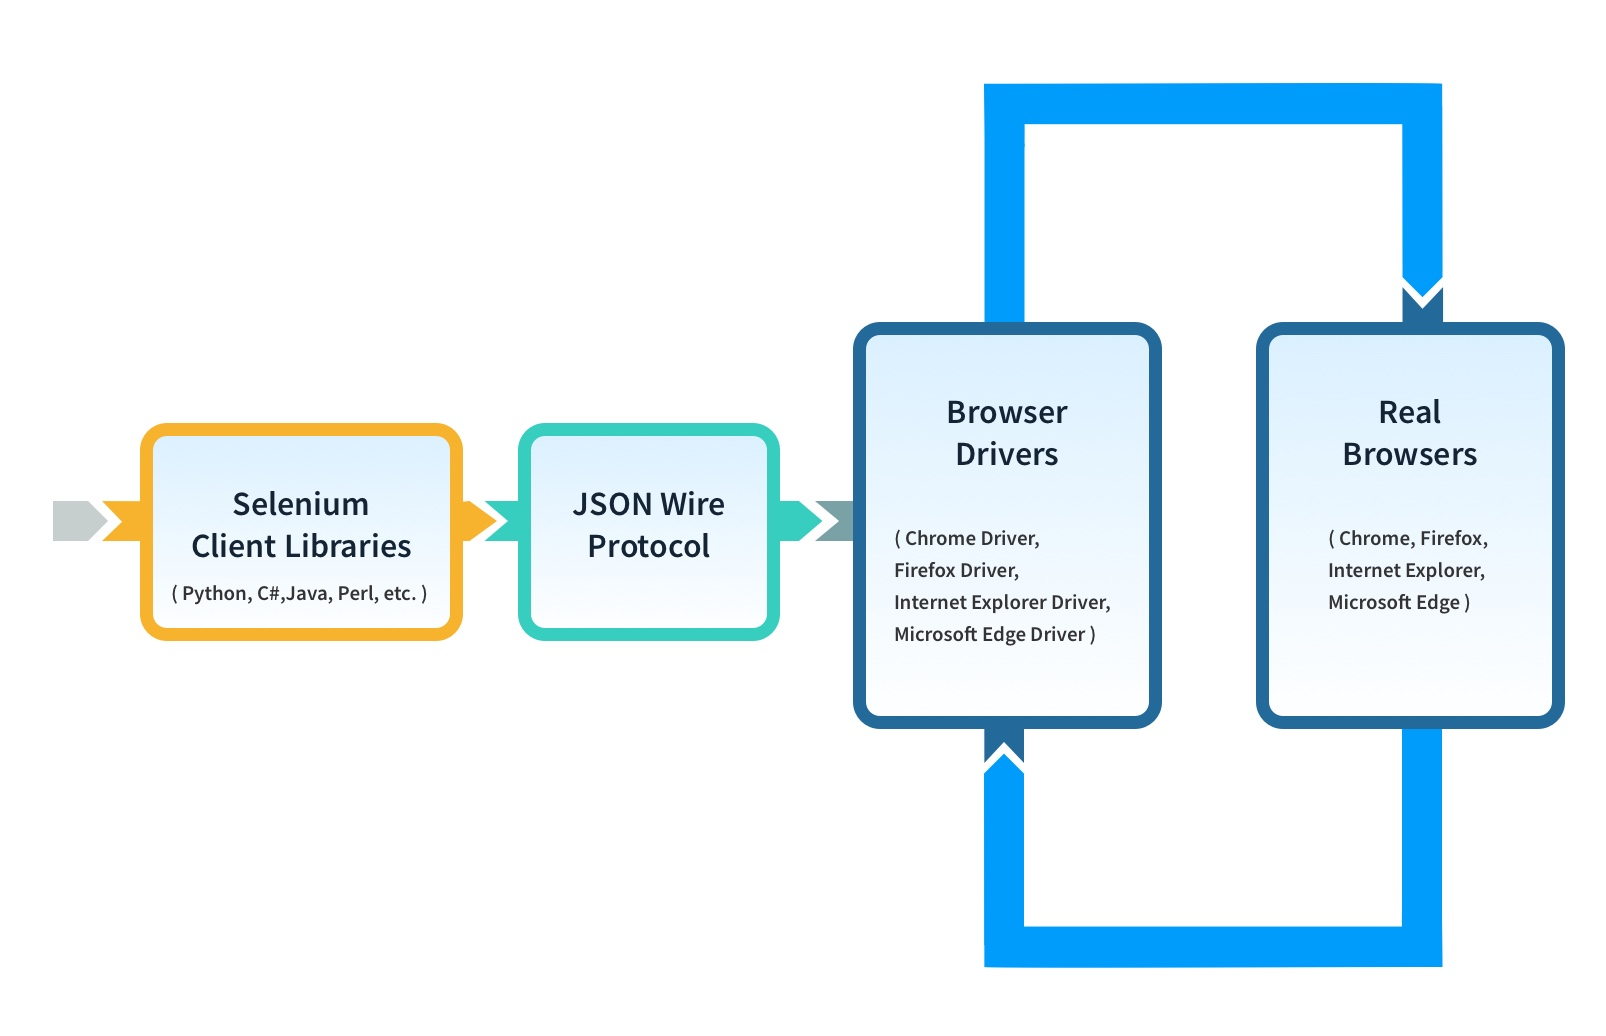
\includegraphics[width=\linewidth]{./images/image8.png}
		\caption{Thành phần chính của WebDriver}
	\end{figure}

	\subsubsection{Ưu điểm}
	
	\begin{itemize}
		\item Là một trong những công cụ kiểm thử mã nguồn mở phổ biến nhất và rất dễ bắt đầu để kiểm thử các ứng dụng web, cho phép thực hiện kiểm thử tự động
		\item Hỗ trợ nhiều hệ điều hành như Windows, Mac, Linux, Unix,...
		\item Hỗ trợ cho các trình duyệt hiện đại như Microsoft Edge, Google Chrome, Firefox, Opera, Safari,...
		\item Cung cấp khả năng tương thích với một số ngôn ngữ lập trình như Python, Java, Perl, Ruby,...
		\item Tốc độ của Selenium WebDriver nhanh hơn một số công cụ kiểm thử tự động khác do giao tiếp trực tiếp với trình duyệt
		\item API ngắn gọn hơn so với Selenium Remote Control
		\item Cung cấp khả năng tương thích với iPhoneDriver, AndroidDriver và HtmlUnitDriver
	\end{itemize}

	\subsubsection{Nhược điểm}
	
	\begin{itemize}
		\item Không có lệnh tích hợp để tạo kết quả kiểm thử tự động
		\item Cần có hiểu biết cơ bản về ngôn ngữ lập trình
		\item Không thể kiểm thử tự động Audio và Video
		\item Cài đặt phức tạp, cần có công cụ để viết mã
	\end{itemize}
	
	\subsection{Selenium Grid}
	
	Selenium Grid là một proxy server thông minh giúp người dùng dễ dàng thực thi các bộ kiểm thử song song trên nhiều thiết bị và trình duyệt khác nhau. Việc kiểm thử được thực hiện bằng cách định tuyến các lệnh đến các trình duyệt web từ xa. Các thiết bị được sử dụng để kiểm thử không nhất thiết phải lưu trữ hard code do Selenium Grid sử dụng chế độ phân tán, chỉ với 1 code base duy nhất là có thể hoạt động được.
	
	Selenium Grid được tạo thành từ hai thành phần chính: hub và node.
	
	\begin{description}
		\item[Hub] máy chủ server, chứa hard code và là nơi nhận các yêu cầu truy cập từ WebDriver client, định tuyến các lệnh kiểm thử đến các Nodes. Hub chỉ có thể được cài đặt duy nhất trên một máy tính.
		\item[Node] những thiết bị bao gồm một hệ điều hành gốc và một WebDriver từ xa được kết nối vào Hub để thực thi các kịch bản kiểm thử. Có thể có nhiều Nodes trong một mô hình Grid.
	\end{description}

	\begin{figure}[H]
		\centering
		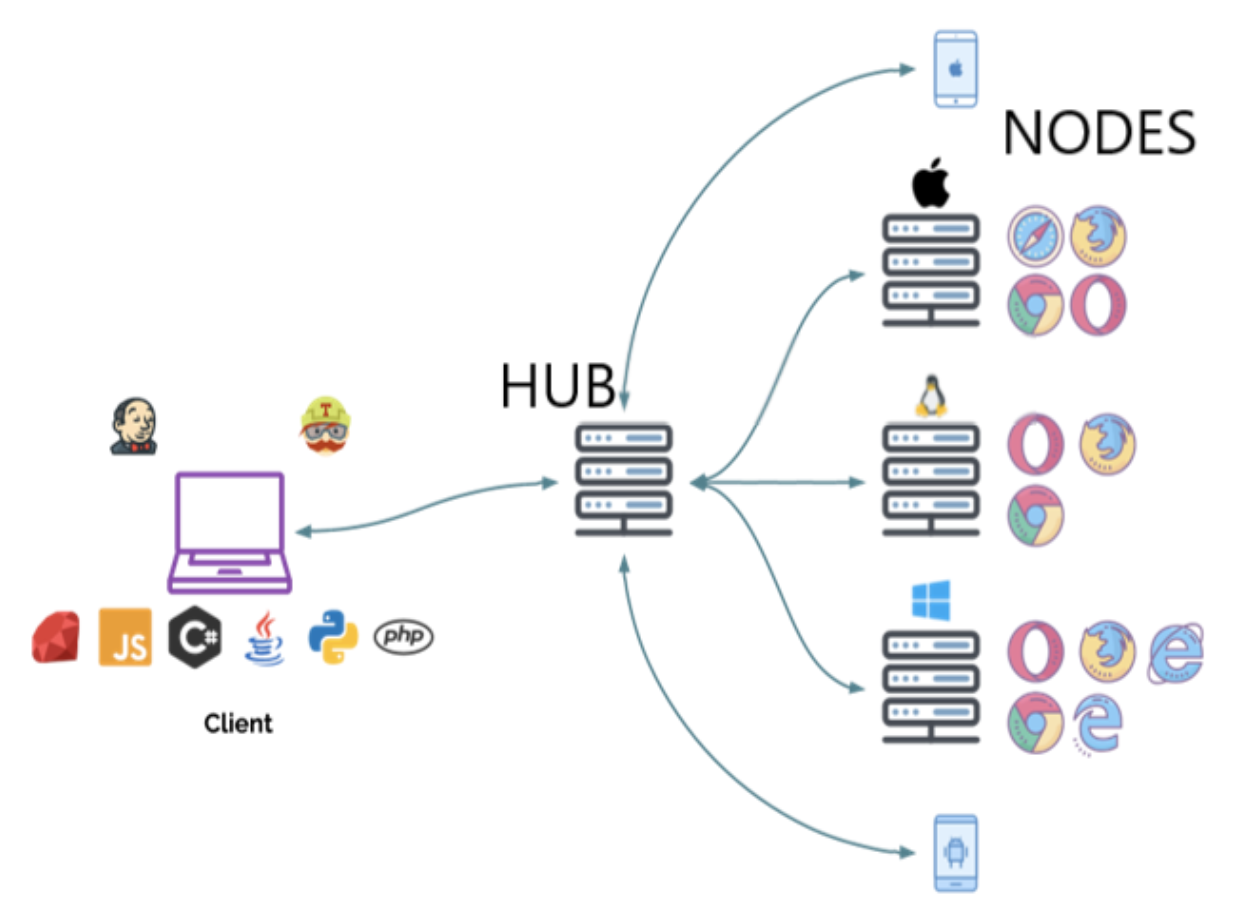
\includegraphics[width=0.8\linewidth]{./images/image3.png}
		\caption{Kiến trúc Selenium Grid}
	\end{figure}

	Người kiểm thử nên sử dụng Selenium Grid trong các trường hợp:
	
	\begin{itemize}
		\item Chạy kiểm thử trên nhiều trình duyệt, thiết bị và hệ điều hành khác nhau và các phiên bản của chúng.
		\item Giảm thời gian mà một bộ kiểm thử cần hoàn thành.
	\end{itemize}
	
	Selenium Grid cải thiện chu kỳ thời gian của các kết quả thử nghiệm. Sự khác biệt này xảy ra là đáng kể, đặc biệt là khi bộ kiểm thử lớn và cần nhiều thời gian hơn để chạy. Nó cung cấp tính linh hoạt và mở rộng phạm vi thử nghiệm trong một thời gian giới hạn. Kể từ khi đưa cơ sở hạ tầng ảo vào sử dụng, việc bảo trì trở nên dễ dàng hơn rất nhiều.

	\subsubsection{Ưu điểm}
	
	\begin{itemize}
		\item Mã nguồn mở, cho phép thực hiện kiểm thử tự động, tương thích với nhiều trình duyệt, hệ điều hành, hỗ trợ nhiều ngôn ngữ lập trình
		\item Tăng thời gian hoàn thành bộ kiểm thử vì khả năng chạy kiểm thử song song
		\item Thực thi trên đám mây, tăng tính khả dụng, độ tin cậy, tiết kiệm chi phí bảo trì phần cứng và phần mềm
	\end{itemize}
	
	\subsubsection{Nhược điểm}
	
	\begin{itemize}
		\item Gia tăng chi phí cho dự án do yêu cầu các thiết bị kiểm thử làm Nodes
		\item Khả năng mở rộng kém, gần như không thể tăng hoặc giảm quy mô theo yêu cầu
		\item Phải cấu hình lại khi có thay đổi do máy chủ được cấu hình trước với một tập hợp các phiên bản trình duyệt bắt buộc có sẵn
		\item Bảo mật kém, yêu cầu người kiểm thử có tay nghề cao thì mới có thể tạo ra và bảo trì nó
	\end{itemize}
	
	\subsection{So sánh với các bộ công cụ khác}
	
	\begin{table}[H]
		\begin{tabular}{p{0.2\textwidth}p{0.2\textwidth}p{0.2\textwidth}p{0.2\textwidth}p{0.2\textwidth}}
			\hline
			\multicolumn{1}{l}{} & \textbf{Selenium} & \textbf{Katalon Studio} & \textbf{UFT} & \textbf{TestComplete} \\ \hline
			\textbf{Hệ điều hành} & Cross-platform & Cross-platform & Windows & Windows \\
			\textbf{Ứng dụng kiểm thử} & Web, Mobile (với Appium) & Web, Mobile, Desktop & Web, Mobile, Desktop & Web, Mobile, Desktop \\
			\textbf{Ngôn ngữ kịch bản} & Java, C\#, Perl, Python, JavaScript, Ruby, PHP & Java, Groovy & VBScript & JavaScript, Python, VBScript, JScript, Delphi, C++, C\# \\
			\textbf{Kỹ năng lập trình} & Có yêu cầu & Không yêu cầu & Không yêu cầu & Không yêu cầu \\
			\textbf{Cài đặt và sử dụng} & Yêu cầu cài đặt một số công cụ & Dễ & Dễ & Dễ \\
			\textbf{Thời gian tạo script} & Chậm & Nhanh & Nhanh & Nhanh \\
			\textbf{Lưu trữ và bảo trì} & XPath, UI Maps & Built-in object repository, XPath, object re-identification & Built-in object repository, smart object detection and correction & Built-in object repository, detecting common objects \\
			\textbf{Kiểm thử dựa trên hình ảnh} & Yêu cầu thư viện ngoài & Hỗ trợ tích hợp & Hỗ trợ tích hợp & Hỗ trợ tích hợp \\
			\textbf{Tích hợp DevOps/ALM} & Yêu cầu thư viện ngoài & Có & Có & Có \\
			\textbf{Tích hợp liên tục} & Jenkins, Cruise Control & Jenkins, Teamcity & Jenkins, HP Quality Center & Jenkins, HP Quality Center \\
			\textbf{Phân tích kiểm thử} & Không & Có & Có & Có \\
			\textbf{Giấy phép} & Mã nguồn mở & Độc quyền & Độc quyền & Độc quyền \\
			\textbf{Chi phí} & Miễn phí & Có phí & Có phí & Có phí \\ \hline
		\end{tabular}
	\end{table}
	
	
\end{document}